% !TEX program = xelatex
\documentclass[a4paper,10pt]{article}
\usepackage[UTF8,fontset=none]{ctex}
\usepackage{xeCJK}
\setCJKmainfont{Songti SC}
\setCJKsansfont{STHeiti}
\setCJKmonofont{Songti SC}
\usepackage[margin=2.2cm]{geometry}
\usepackage{tikz}
\usetikzlibrary{shapes.geometric, arrows.meta, positioning, calc, fit}
\usepackage{amsmath, amssymb}
\usepackage{longtable}
\usepackage{array}
\usepackage{booktabs}
\usepackage{multirow}
\usepackage{enumitem}
\usepackage{fancyhdr}
\usepackage{titlesec}
\usepackage{hyperref}
\usepackage{xcolor}
\usepackage{tabularx}

\hypersetup{
  colorlinks=true,
  linkcolor=blue!60!black,
  urlcolor=blue!60!black,
  bookmarksnumbered=true
}

\pagestyle{fancy}
\fancyhf{}
\fancyhead[L]{\small fitCubicPolynomial 函数设计文档}
\fancyhead[R]{\small 内部公开}
\fancyfoot[C]{\thepage}
\renewcommand{\headrulewidth}{0.4pt}

\setcounter{secnumdepth}{3}
\setcounter{tocdepth}{3}

\newcolumntype{L}[1]{>{\raggedright\arraybackslash}p{#1}}
\newcolumntype{C}[1]{>{\centering\arraybackslash}p{#1}}

% ============================================================
\begin{document}

% ==================== 封面表格 ====================
\thispagestyle{empty}

\begin{center}
{\CJKfamily{zhsong}\bfseries\Large 函数设计文档}
\end{center}

\vspace{8pt}

\begin{center}
\renewcommand{\arraystretch}{1.5}
\begin{tabular}{|L{3.2cm}|L{4.5cm}|L{3.2cm}|L{4.5cm}|}
\hline
\textbf{函数英文名} & fitCubicPolynomial &
\textbf{函数中文名} & 三次多项式拟合 \\
\hline
\textbf{函数类型} & 元件 (Element) &
\textbf{版本} & 2.0 \\
\hline
\textbf{作者} & 许庆 &
\textbf{日期} & 2026-06-26 \\
\hline
\textbf{联系方式} & \multicolumn{3}{l|}{18612426814~/~qingxu@tsinghua.edu.cn} \\
\hline
\textbf{密级} & 内部公开 &
\textbf{AI辅助} & Cursor Agent (Claude Opus 4.6) \\
\hline
\end{tabular}
\end{center}

\vspace{12pt}

\begin{center}
\renewcommand{\arraystretch}{1.4}
\begin{tabular}{|C{1cm}|C{1.8cm}|L{3.8cm}|C{1.5cm}|C{1.5cm}|C{3cm}|}
\hline
\multicolumn{6}{|c|}{\textbf{更改记录}} \\
\hline
\textbf{版本} & \textbf{日期} & \textbf{更改说明} & \textbf{作者} & \textbf{审核} & \textbf{辅助AI} \\
\hline
1.0 & 2026-06-20 & 初始版本 & 许庆 & --- & --- \\
\hline
2.0 & 2026-06-26 & 重构为法方程 + 高斯消元 & 许庆 & --- & Claude Opus 4.6 \\
\hline
\end{tabular}
\end{center}

\newpage

% ==================== 目录 ====================
\tableofcontents
\newpage

% ============================================================
%  1. 函数需求
% ============================================================
\section{函数需求}

\subsection{功能概述}

\texttt{fitCubicPolynomial} 对给定数据点 $(x_i, y_i)$ 进行三次多项式最小二乘拟合，
求解系数 $c_0, c_1, c_2, c_3$ 使得
$y(x) = c_0 + c_1 x + c_2 x^2 + c_3 x^3$
在最小二乘意义下最优逼近数据。
内部通过构造 Vandermonde 法方程并调用 \texttt{solveLinearSystem} 求解。

\subsection{输入/输出/返回值}

\renewcommand{\arraystretch}{1.3}
\begin{longtable}{|L{2.2cm}|L{3cm}|C{2.5cm}|L{7cm}|}
\hline
\textbf{方向} & \textbf{名称} & \textbf{类型} & \textbf{说明} \\
\hline
\endfirsthead
\hline
\textbf{方向} & \textbf{名称} & \textbf{类型} & \textbf{说明} \\
\hline
\endhead
输入 & \texttt{xData} & \texttt{const double*} & X 坐标数组（\texttt{numPoints} 个元素） \\
\hline
输入 & \texttt{yData} & \texttt{const double*} & Y 坐标数组（\texttt{numPoints} 个元素） \\
\hline
输入 & \texttt{numPoints} & \texttt{const int} & 数据点数量（需 $\geq 4$） \\
\hline
返回值 & --- & \texttt{PolynomialCoeffs} & 拟合系数 $\mathbf{c} = [c_0, c_1, c_2, c_3]$；求解失败时系数全零 \\
\hline
\end{longtable}

\subsection{功能需求}

\begin{enumerate}[label=FR-\arabic*]
  \item 构造三次 Vandermonde 矩阵 $\mathbf{A}$ 对应的法方程 $\mathbf{A}^{\!\top}\!\mathbf{A}\,\mathbf{c} = \mathbf{A}^{\!\top}\!\mathbf{y}$。
  \item 调用 \texttt{solveLinearSystem} 求解 $4 \times 4$ 法方程。
  \item 求解成功时将系数存入返回结构体；失败时系数保持默认零值。
  \item 支持数据点数量 $m \geq 4$ 的过定系统。
\end{enumerate}

\subsection{非功能需求}

\begin{enumerate}[label=NFR-\arabic*]
  \item 不使用动态内存分配，法方程矩阵使用 \texttt{MAX\_LINEAR\_SYSTEM\_DIM} 大小的静态数组。
  \item 不依赖第三方线性代数库。
  \item 时间复杂度 $O(m)$（法方程组装）$+$ $O(1)$（$4 \times 4$ 系统求解）。
\end{enumerate}

% ============================================================
%  2. 算法设计
% ============================================================
\section{算法设计}

\subsection{最小二乘问题建模}

给定 $m$ 个数据点 $(x_i, y_i)$，$i = 0, 1, \ldots, m{-}1$，
寻找三次多项式系数 $\mathbf{c} = [c_0, c_1, c_2, c_3]^{\!\top}$ 使残差平方和最小：
\begin{equation}
  \min_{\mathbf{c}} \sum_{i=0}^{m-1} \bigl(c_0 + c_1 x_i + c_2 x_i^2 + c_3 x_i^3 - y_i\bigr)^2
  = \min_{\mathbf{c}} \|\mathbf{A}\mathbf{c} - \mathbf{y}\|_2^2
\end{equation}

\subsection{Vandermonde 矩阵}

构造 $m \times 4$ 的 Vandermonde 矩阵 $\mathbf{A}$：
\begin{equation}
  \mathbf{A} = \begin{bmatrix}
    1 & x_0 & x_0^2 & x_0^3 \\
    1 & x_1 & x_1^2 & x_1^3 \\
    \vdots & \vdots & \vdots & \vdots \\
    1 & x_{m-1} & x_{m-1}^2 & x_{m-1}^3
  \end{bmatrix}, \quad
  \mathbf{y} = \begin{bmatrix} y_0 \\ y_1 \\ \vdots \\ y_{m-1} \end{bmatrix}
\end{equation}

在代码实现中，并不显式构造 $\mathbf{A}$，而是逐点累加构造法方程。

\subsection{法方程推导}

对目标函数 $J(\mathbf{c}) = \|\mathbf{A}\mathbf{c} - \mathbf{y}\|_2^2$ 求导并令其为零：
\begin{equation}
  \frac{\partial J}{\partial \mathbf{c}} = 2\mathbf{A}^{\!\top}(\mathbf{A}\mathbf{c} - \mathbf{y}) = \mathbf{0}
\end{equation}
得到法方程（Normal Equations）：
\begin{equation}\label{eq:normal}
  \boxed{\mathbf{A}^{\!\top}\!\mathbf{A}\,\mathbf{c} = \mathbf{A}^{\!\top}\!\mathbf{y}}
\end{equation}
其中 $\mathbf{A}^{\!\top}\!\mathbf{A}$ 为 $4 \times 4$ 对称半正定矩阵，各元素为：
\begin{equation}
  (\mathbf{A}^{\!\top}\!\mathbf{A})_{jk} = \sum_{i=0}^{m-1} x_i^{\,j+k}, \quad j, k = 0, 1, 2, 3
\end{equation}
右端向量各元素为：
\begin{equation}
  (\mathbf{A}^{\!\top}\!\mathbf{y})_j = \sum_{i=0}^{m-1} x_i^{\,j} \cdot y_i, \quad j = 0, 1, 2, 3
\end{equation}

\subsection{逐点累加实现}

对每个数据点 $(x_i, y_i)$，构造幂向量 $\mathbf{p}_i = [1, x_i, x_i^2, x_i^3]^{\!\top}$，然后：
\begin{equation}
  \mathbf{A}^{\!\top}\!\mathbf{A} \mathrel{+}= \mathbf{p}_i \mathbf{p}_i^{\!\top}, \quad
  \mathbf{A}^{\!\top}\!\mathbf{y} \mathrel{+}= y_i \cdot \mathbf{p}_i
\end{equation}

组装完成后，调用 \texttt{solveLinearSystem(ata, aty, 4, MAX\_LINEAR\_SYSTEM\_DIM)} 求解系数。

% ============================================================
%  3. 程序流程图
% ============================================================
\section{程序流程图}

\begin{center}
\begin{tikzpicture}[
  node distance=0.9cm and 2cm,
  startstop/.style={rectangle, rounded corners, minimum width=3.5cm, minimum height=0.7cm,
    text centered, draw=black, fill=blue!8, font=\small},
  process/.style={rectangle, minimum width=5cm, minimum height=0.7cm,
    text centered, draw=black, fill=orange!8, font=\small},
  decision/.style={diamond, aspect=2.5, minimum width=2cm,
    text centered, draw=black, fill=green!8, font=\small},
  io/.style={trapezium, trapezium left angle=70, trapezium right angle=110,
    minimum width=3.5cm, minimum height=0.7cm,
    text centered, draw=black, fill=yellow!8, font=\small},
  subcall/.style={rectangle, minimum width=4.5cm, minimum height=0.7cm,
    text centered, draw=black, fill=cyan!8, font=\small,
    double, double distance=1.5pt},
  arrow/.style={-{Stealth[length=2.5mm]}, thick}
]

\node (start) [startstop] {开始};
\node (input) [io, below=of start] {读入 xData, yData, numPoints};
\node (init) [process, below=of input] {初始化 $\mathbf{A}^{\!\top}\!\mathbf{A} = \mathbf{0}$, $\mathbf{A}^{\!\top}\!\mathbf{y} = \mathbf{0}$};
\node (loop) [decision, below=of init] {$i < $ numPoints?};
\node (xpow) [process, below=of loop] {构造 $\mathbf{p}_i = [1, x_i, x_i^2, x_i^3]$};
\node (accum) [process, below=of xpow] {累加 $\mathbf{A}^{\!\top}\!\mathbf{A}$, $\mathbf{A}^{\!\top}\!\mathbf{y}$};
\node (inc) [process, below=of accum] {$i \gets i + 1$};
\node (solve) [subcall, below=1.5cm of inc] {solveLinearSystem(ata, aty, 4, maxDim)};
\node (chk) [decision, below=of solve] {求解成功?};
\node (copy) [process, below=of chk] {复制系数到 result.c[]};
\node (zero) [process, right=3cm of chk] {系数保持全零};
\node (output) [io, below=of copy] {输出 PolynomialCoeffs};
\node (stop) [startstop, below=of output] {结束};

\draw [arrow] (start) -- (input);
\draw [arrow] (input) -- (init);
\draw [arrow] (init) -- (loop);
\draw [arrow] (loop) -- node[right]{\small 是} (xpow);
\draw [arrow] (xpow) -- (accum);
\draw [arrow] (accum) -- (inc);
\draw [arrow] (inc.west) -- ++(-2,0) |- (loop.west);
\draw [arrow] (loop.east) -- ++(2,0) node[above,midway]{\small 否} |- (solve.east);
\draw [arrow] (solve) -- (chk);
\draw [arrow] (chk) -- node[right]{\small 是} (copy);
\draw [arrow] (chk) -- node[above]{\small 否} (zero);
\draw [arrow] (zero) |- (output);
\draw [arrow] (copy) -- (output);
\draw [arrow] (output) -- (stop);

\end{tikzpicture}
\end{center}

% ============================================================
%  4. 函数接口与输入输出模块图
% ============================================================
\section{函数接口与输入输出模块图}

\subsection{函数接口}

\begin{verbatim}
PolynomialCoeffs fitCubicPolynomial(const double* xData,
                                     const double* yData,
                                     const int numPoints);
\end{verbatim}

\subsection{输入输出模块图}

\begin{center}
\begin{tikzpicture}[
  core/.style={rectangle, draw=black, very thick, minimum width=5cm, minimum height=2cm,
    text centered, fill=orange!10, font=\normalsize\bfseries, rounded corners=3pt},
  iobox/.style={rectangle, draw=black, thick, minimum width=3.2cm, minimum height=0.6cm,
    text centered, fill=yellow!10, font=\small},
  arrow/.style={-{Stealth[length=2.5mm]}, thick}
]

\node (core) [core] {fitCubicPolynomial};

\node (in1) [iobox, left=3cm of core, yshift=0.8cm] {xData (const double*)};
\node (in2) [iobox, left=3cm of core, yshift=0cm] {yData (const double*)};
\node (in3) [iobox, left=3cm of core, yshift=-0.8cm] {numPoints (int)};

\node (out1) [iobox, right=3cm of core] {PolynomialCoeffs};

\draw [arrow] (in1) -- (core);
\draw [arrow] (in2) -- (core);
\draw [arrow] (in3) -- (core);
\draw [arrow] (core) -- (out1);

\node [above=0.1cm of in1, font=\small\bfseries] {输入 (Input)};
\node [above=0.1cm of out1, font=\small\bfseries] {输出 (Output)};

\end{tikzpicture}
\end{center}

% ============================================================
%  5. 函数诸元表
% ============================================================
\section{函数诸元表}

\renewcommand{\arraystretch}{1.3}
\begin{longtable}{|L{3.8cm}|L{11.5cm}|}
\hline
\textbf{属性} & \textbf{说明} \\
\hline
\endfirsthead
\hline
\textbf{属性} & \textbf{说明} \\
\hline
\endhead
函数英文名 & \texttt{fitCubicPolynomial} \\
\hline
函数中文名 & 三次多项式拟合 \\
\hline
函数类型 & 元件 (Element) \\
\hline
版本 & 2.0 \\
\hline
源文件 & \texttt{src/cpp/fitCubicPolynomial/fitCubicPolynomial.cpp} \\
\hline
头文件 & \texttt{include/cpp/fitCubicPolynomial/fitCubicPolynomial.hpp} \\
\hline
命名空间 & \texttt{waypoint\_follow} \\
\hline
输入数量 & 3（xData, yData, numPoints） \\
\hline
输出数量 & 1（PolynomialCoeffs 返回值） \\
\hline
参数数量 & 0 \\
\hline
状态数量 & 0 \\
\hline
下级函数数量 & 1（solveLinearSystem） \\
\hline
动态内存分配 & 无 \\
\hline
外部依赖 & 无（间接依赖 \texttt{<cmath>} 经由 solveLinearSystem） \\
\hline
算法类别 & 最小二乘拟合 / 法方程法 \\
\hline
时间复杂度 & $O(m)$（法方程组装，$m$ 为数据点数）$+$ $O(1)$（$4{\times}4$ 系统求解） \\
\hline
多项式阶数 & 3（系数数量 $= \texttt{POLY\_COEFFS\_NUM} = 4$） \\
\hline
\end{longtable}

% ============================================================
%  6. 函数架构图
% ============================================================
\section{函数架构图}

\begin{center}
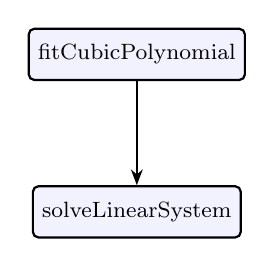
\begin{tikzpicture}[
  every node/.style={rectangle, draw, rounded corners=2pt, thick,
    minimum height=0.65cm, text centered, font=\footnotesize,
    fill=blue!5},
  edge from parent/.style={draw, -{Stealth[length=2mm]}, thick},
  level 1/.style={level distance=2.0cm}
]

\node {fitCubicPolynomial}
  child { node {solveLinearSystem} };

\end{tikzpicture}
\end{center}

% ============================================================
%  7. 下级函数需求
% ============================================================
\section{下级函数需求}

\subsection{solveLinearSystem~---~线性方程组求解}

\begin{itemize}
  \item \textbf{功能}：使用高斯消元法（部分主元选取）求解 $n \times n$ 线性方程组 $\mathbf{A}\mathbf{x} = \mathbf{b}$。
  \item \textbf{输入}：
    \begin{itemize}
      \item \texttt{matrix} (\texttt{double*})：行主序系数矩阵，求解过程中被修改。
      \item \texttt{rhs} (\texttt{double*})：右端向量，求解后存放解向量。
      \item \texttt{n} (\texttt{int})：方程组维数。
      \item \texttt{maxDim} (\texttt{int})：矩阵行步长。
    \end{itemize}
  \item \textbf{输出}：\texttt{bool} --- 求解成功返回 \texttt{true}，矩阵奇异返回 \texttt{false}。
  \item \textbf{调用方式}：\texttt{solveLinearSystem(ata, aty, 4, MAX\_LINEAR\_SYSTEM\_DIM)}。
    其中 \texttt{ata} 为 $4 \times 4$ 法方程矩阵 $\mathbf{A}^{\!\top}\!\mathbf{A}$，
    \texttt{aty} 为法方程右端向量 $\mathbf{A}^{\!\top}\!\mathbf{y}$。
  \item \textbf{异常处理}：当法方程矩阵奇异（数据点退化）时返回 \texttt{false}，
    \texttt{fitCubicPolynomial} 据此返回全零系数。
\end{itemize}

% ============================================================
%  8. 数据结构定义
% ============================================================
\section{数据结构定义}

以下数据结构定义于 \texttt{waypointFollowTypes.hpp}，命名空间 \texttt{waypoint\_follow}。

\subsection{常量定义}

\begin{longtable}{|L{5cm}|C{1.5cm}|L{8.5cm}|}
\hline
\textbf{常量名} & \textbf{值} & \textbf{说明} \\
\hline
\texttt{POLY\_COEFFS\_NUM} & 4 & 三次多项式系数数量（阶数 $+ 1$） \\
\hline
\texttt{MAX\_LINEAR\_SYSTEM\_DIM} & 8 & 线性方程组求解器最大维数 \\
\hline
\end{longtable}

\subsection{PolynomialCoeffs~---~三次多项式系数}

\begin{longtable}{|L{3.5cm}|C{2cm}|L{9.5cm}|}
\hline
\textbf{成员} & \textbf{类型} & \textbf{说明} \\
\hline
\texttt{c[4]} & double[4] & $y = c_0 + c_1 x + c_2 x^2 + c_3 x^3$；默认初始化为全零 \\
\hline
\end{longtable}

当 \texttt{solveLinearSystem} 返回 \texttt{false} 时，系数保持默认零值，
可据此隐式判断拟合是否成功。

% ============================================================
%  9. 测试用例
% ============================================================
\section{测试用例}

\subsection{正常测试用例}

{\small
\begin{longtable}{|C{0.6cm}|L{1.8cm}|L{5.0cm}|L{3.8cm}|L{3.5cm}|}
\hline
\textbf{编号} & \textbf{场景} & \textbf{输入} & \textbf{预期输出} & \textbf{验证准则} \\
\hline
\endfirsthead
\hline
\textbf{编号} & \textbf{场景} & \textbf{输入} & \textbf{预期输出} & \textbf{验证准则} \\
\hline
\endhead
N-1 &
精确三次数据 &
$\mathbf{x}{=}[0,1,2,3,4]$, $y_i{=}1{+}2x_i{+}3x_i^2{+}4x_i^3$, $m{=}5$ &
$\mathbf{c}{=}[1,2,3,4]$ &
$\|\mathbf{c} - \mathbf{c}^*\|_\infty < 10^{-8}$ \\
\hline
N-2 &
二次数据 &
$\mathbf{x}{=}[0,1,2,3,4]$, $y_i{=}x_i^2$, $m{=}5$ &
$\mathbf{c}{\approx}[0,0,1,0]$ &
$|c_3| < 10^{-10}$, $|c_2 - 1| < 10^{-10}$ \\
\hline
N-3 &
线性数据 &
$\mathbf{x}{=}[0,1,2,3,4]$, $y_i{=}2x_i{+}1$, $m{=}5$ &
$\mathbf{c}{\approx}[1,2,0,0]$ &
$|c_2|, |c_3| < 10^{-10}$ \\
\hline
N-4 &
常数数据 &
$\mathbf{x}{=}[0,1,2,3,4]$, $y_i{=}5$, $m{=}5$ &
$\mathbf{c}{\approx}[5,0,0,0]$ &
$|c_0 - 5| < 10^{-10}$ \\
\hline
N-5 &
过定系统 &
$\mathbf{x}{=}[{-}2,{-}1,0,1,2,3]$, $y_i{=}x_i^3$, $m{=}6$ &
$\mathbf{c}{\approx}[0,0,0,1]$ &
精确三次数据的过定拟合 \\
\hline
\end{longtable}
}

\vspace{6pt}
{\small
\begin{longtable}{|L{2.8cm}|L{12.5cm}|}
\hline
\multicolumn{2}{|c|}{\textbf{正常测试用例符号说明}} \\
\hline
\textbf{符号} & \textbf{含义} \\
\hline
$\mathbf{x}$ & X 坐标数组 xData \\
\hline
$y_i$ & 第 $i$ 个 Y 坐标 yData[$i$] \\
\hline
$m$ & 数据点数量 numPoints \\
\hline
$\mathbf{c}{=}[c_0,c_1,c_2,c_3]$ & 拟合系数 PolynomialCoeffs.c[] \\
\hline
$\mathbf{c}^*$ & 理论精确系数 \\
\hline
$\|\cdot\|_\infty$ & 向量无穷范数 \\
\hline
\end{longtable}
}

\subsection{异常测试用例}

{\small
\begin{longtable}{|C{0.6cm}|L{1.8cm}|L{4.8cm}|L{3.8cm}|L{3.5cm}|}
\hline
\textbf{编号} & \textbf{场景} & \textbf{输入} & \textbf{预期输出/行为} & \textbf{验证准则} \\
\hline
\endfirsthead
\hline
\textbf{编号} & \textbf{场景} & \textbf{输入} & \textbf{预期输出/行为} & \textbf{验证准则} \\
\hline
\endhead
A-1 &
$x$ 全相同 &
$x_i{=}1$ ($\forall i$), $m{=}5$ &
法方程奇异, $\mathbf{c}{=}[0,0,0,0]$ &
$\mathbf{A}^{\!\top}\!\mathbf{A}$ 秩为 1 \\
\hline
A-2 &
$m{=}0$ &
空数组, $m{=}0$ &
$\mathbf{A}^{\!\top}\!\mathbf{A} = \mathbf{0}$, $\mathbf{c}{=}\mathbf{0}$ &
零数据点 → 全零矩阵 \\
\hline
A-3 &
$m{=}1$ &
$(x_0, y_0){=}(2, 5)$, $m{=}1$ &
$\mathbf{A}^{\!\top}\!\mathbf{A}$ 秩为 1, $\mathbf{c}{=}\mathbf{0}$ &
欠定: 单点无唯一解 \\
\hline
A-4 &
xData 含 NaN &
$x_2{=}\text{NaN}$, 其余正常 &
不崩溃; $\mathbf{c}$ 可能全零或含 NaN &
函数正常返回 \\
\hline
A-5 &
yData 含 NaN &
$y_1{=}\text{NaN}$, 其余正常 &
不崩溃; $\mathbf{c}$ 可能含 NaN &
函数正常返回 \\
\hline
A-6 &
xData 含 $+\infty$ &
$x_0{=}+\infty$, 其余正常 &
不崩溃; 法方程含 $\infty$ &
无浮点异常 \\
\hline
A-7 &
yData 含 $+\infty$ &
$y_3{=}+\infty$, 其余正常 &
不崩溃; $\mathbf{A}^{\!\top}\mathbf{y}$ 含 $\infty$ &
无浮点异常 \\
\hline
A-8 &
$x$ 全为零 &
$x_i{=}0$ ($\forall i$), $y_i$ 各异, $m{=}5$ &
$\mathbf{A}^{\!\top}\!\mathbf{A}$ 秩为 1, $\mathbf{c}{=}\mathbf{0}$ &
$\mathbf{p}_i{=}[1,0,0,0]$ \\
\hline
A-9 &
$x$ 间距极小 &
$x_i{=}i \times 10^{-15}$, $m{=}5$ &
法方程接近奇异; $\mathbf{c}$ 精度退化或全零 &
条件数极大 \\
\hline
A-10 &
$m{=}3$（欠定） &
3 个不同数据点, $m{=}3$ &
$\mathbf{A}^{\!\top}\!\mathbf{A}$ 秩 $\leq 3$, 可能奇异 &
$4 \times 4$ 矩阵秩不足 \\
\hline
\end{longtable}
}

\vspace{6pt}
{\small
\begin{longtable}{|L{2.8cm}|L{12.5cm}|}
\hline
\multicolumn{2}{|c|}{\textbf{异常测试用例符号说明}} \\
\hline
\textbf{符号} & \textbf{含义} \\
\hline
$x_i$ & 第 $i$ 个 X 坐标 xData[$i$] \\
\hline
$y_i$ & 第 $i$ 个 Y 坐标 yData[$i$] \\
\hline
$m$ & 数据点数量 numPoints \\
\hline
$\mathbf{c}$ & 拟合系数 PolynomialCoeffs.c[] \\
\hline
$\mathbf{A}^{\!\top}\!\mathbf{A}$ & $4 \times 4$ 法方程系数矩阵 \\
\hline
$\mathbf{p}_i$ & 第 $i$ 个数据点的幂向量 $[1, x_i, x_i^2, x_i^3]$ \\
\hline
NaN & IEEE 754 非数值 (Not a Number) \\
\hline
$+\infty$ & IEEE 754 正无穷大 \\
\hline
\end{longtable}
}

\end{document}
